\chapter{Electrospray ionization source}
\label{chap:ESI}

\section{Overview of the electrospray and its components}
As the source of molecular ions for the experiment we implement a so-called electrospray ionization (ESI) source \cite{FennEsi,Kjaer2021-lm}. At the time of writing, the ESI source is not connected to the rest of the setup, but an illustration of what the setup will look like when everything is connected can be seen on \cref{fig:fullSetup}.
\begin{figure}
    \centering
    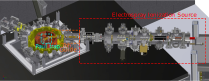
\includegraphics[width = 1.1\textwidth]{main/spray.pdf}
    \caption{3D figure of the full setup at Aarhus, when the electrospray (red) is connected to the cryogenic trap. The ion guide (orange) allows to transfer the ions into the cryogenic Paul trap (blue), where experiments will be conducted. At the time of writing the ESI source is not hooked up to the experiment, and instead there is channeltron detector at the very end of the electrospray, where it would connect to the ion guide}
    \label{fig:fullSetup}
\end{figure}


The basics of how such a device functions is that it has a syringe contains a solvent (typically methanol) with the ions one wishes to perform experiments on. The syringe is connected to a needle, and a motor slowly depresses the plunger on the spring, causing the solvent to form a droplet on the tip of the needle. The needle tip of the ESI source is sitting outside the vacuum chambers of the ESI setup, in atmospheric air.
Opposite of the needle is a narrow opening into the full body of the ESI source. The tip of the needle is put at a high voltage difference with respect to this opening (typically 3-3.5kV), this voltage difference leads to a strong electric field which will drag the charged droplets from the needle and into the opening of the instrument.
The ions then enter a capillary tube (see \cref{fig:esiDrawing}) heated to 70 degrees celsius, which is set at some voltage (typically 40V).
\begin{figure}
    \centering
    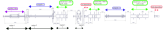
\includegraphics[width = 1.1\textwidth]{main/electrospray_elements.pdf}
    \caption{Technical drawing giving a sideview of all the components of the ESI source we employ. Some of the most important components on the figure have been labelled by name and the voltages typically emplyed on them.
    It is very important to ensure that there is a voltage gradient as one progresses down the ESI source, since otherwise the ions cannot travel. The multiple voltages noted for the Einzel lenses correspond to outer/inner electrode voltages, and for the extraction lens, the low voltage is set for extraction, while the high is for accumulation}
    \label{fig:esiDrawing}
\end{figure}
Within the heated capillary the solvent will begin to evaporate, causing the droplets to shrink. This causes the Coulomb repulsion of the ions within the droplet to increase as they all move nearer one another.
Eventually the surface tension of the droplet can no longer compensate the electrostatic repulsion of the ions within, and the droplet splits. This process repeats until all the solvent is evaporated and the ions are situated in the gas-phase. A schematic of this principle is illustrated on \cref{fig:evaporation}.
\begin{figure}
    \centering
    \includegraphics{main/evaporation.pdf}
    \caption{Illustration of the evaporation principle that allows for gas-phase ions in electrospraying. As the solvent evaporates, the droplet will shrink, until the surface tension becomes unable to counteract the electrostatic repulsion of the ions. This splits the droplet into two droplets, for which this process then repeats. Eventually all the solvent is evaporated and only gas-phase ions are left. Note that the number of ions within a droplet has been grossly underestimated for ease of illustration}
    \label{fig:evaporation}
\end{figure}

After the evaporation process, gas-phase ions travel past a skimmer and into an octopole storage device. The octopole allows for efficient transport of the ions across long regions, and acts as a source of buffer gas cooling down to room temperature, due to ion-neutral collisions with the atmospheric gas at a pressure of approx 1mbar. At the very end of the octopole is a pair of "extraction" electrodes (also called lenses). We have timed control of these electrodes, allowing us to accumulate ions in the octopole by setting a high voltage on them, and then releasing the ion bunch by lowering the voltage. We have performed several experiments on this part of the trap, to characterize the storage capabilities of the octopole, as well as the temporal shape of the ion bunches that arrive from it. The results of those investigations are found in \cref{sec:octopoleExperiments}.

Upon extraction from the octopole the ions pass through an Einzel lens. This is a set of three electrodes, where the outer two share the same voltage, and fulfills the same role for ions as a lens does for optics. We use the Einzel lens to focus down the ion beam onto the 2mm wide opening of a cylindrical Paul trap.

The cylindrical Paul trap has two different settings. The first is using it as an Einzel lens, where the front and back electrodes act as the outer electrodes, while the main cylinder acts as the center electrode. This setting uses no RF on the trap and just allows for a DC ion beam going through.
The other option is to utilize the RF on the Paul trap, in order to trap and store ions. Since we only need a single molecule within the cryogenic trap, we would like to be able to load ions into the Paul trap, and use it as a "secondary" ion source, extracting just a few ions at a time for experiments.
Additionally it is possible to leak in gas for buffer gas cooling of molecules stored in the cylindrical Paul trap.

Immediately after the Paul trap there is a channel electron multiplier detector (also referred to as a channeltron), which can measure the ion current. This detector has a push/pull feedthrough, allowing it to be moved in and out of the ion beam. This allows us to perform diagnostics on the components of the first half of the detector. Of course, if the detector is moved into the ion beam, there will be no ions further down in the setup.

If the first channeltron detector is not in the measurement position, the ions will continue down to another set of Einzel lenses, which focus them into a second octopole that moves them down to a final set of Einzel lenses, focusing them onto a 2nd channeltron detector. This 2nd detector allows us to measure the ion current that makes it all the way through the ESI part of the experiment.
It has to be noted, that the 2nd detector sits where the connection to the ion guide will eventually be mounted, and as such this is not a permanent installation, but only exists for testing parameters to ensure we are able to get ions to the very end of the ESI source.
\section{Experiments on the first octopole}
\label{sec:octopoleExperiments}
The need for getting only single molecular ions in our cryogenic Paul trap poses some very unique challenges for our ESI setup. Since these ion sources are built to maximize the number of ions moving through, we will need to have a very good understanding of the different parts of the electrospray in order to be able to tailor a protocol for getting single ions to our linear quadropole trap.
For this reason we have spent some time making a characterization of the very first octopole in the experiment. 
This section contains the results of these measurements. All measurements are performed on rhodamine 6G, since it sprays particularly well.

\subsection{Measuring the temporal shape of an ion bunch}
One of the first characterizations we perform is measuring the temporal shape of an ion bunch leaving the octopole.

To get such a measurement we allow ions to accumulate in the octopole for some set amount of time by setting the voltage on the extraction lens to 40V, until the ions are released by lowering the voltage to -10V. After some delay $\tau$ with respect to the release of the ions, the number of ions hitting the detector over a time interval of 50$\mu$s is then recorded. By repeating this method for several values of $\tau$ we are able to get a temporal shape of the ion bunch coming out of the octopole.
An illustration of the measurement sequence can be seen on \cref{fig:sequenceShape}. 

Since it is unclear how narrow the ion bunch is in time, the ion signal is adjusted such that when the electrospray is in the DC configuration a current of a few 100 ions per second is measured, this ensures the detector will not saturate.
\begin{figure}
    \centering
    \includegraphics[width = 0.8\textwidth]{main/ShapePulse.pdf}
    \caption{Illustration of the experimental sequence for measuring the temporal shape of ion bunches leaving the first octopole (figure not to scale). Ions are accumulated (blue) over a preset time (data for 500ms, 30sec, and 1 minute were recorded) and then released. The measurement (red) is turned on for 50$\mu$s with a delay $\tau$ with respect to the release of the ions.
    Measurements are repeated 20 times for each value of $\tau$ in order to ensure good statistics. By varying $\tau$ and recording the number of ions a temporal shape of the ion bunch is recorded}
    \label{fig:sequenceShape}
\end{figure}

Results from the measurements when the octopole is allowed to accumulate ions for 500ms, 30 seconds and 1 minute can be seen on 
\cref{fig:bunchShape}. Here three loading times are compared, namely 500ms (green), 30 seconds (blue), and 1 minute (orange).
It is seen that the curves for 30 seconds and 1 minute are highly similar, this is likely because they contain very similar amounts of ions as can be seen on \cref{fig:fillTimeGraph}.

The 500ms curve is considerably slower than the other two, both in its rise time and its tail, by approximately a factor of 2. This indicates that the number of ions seems to affect the temperature, with fewer ions leading to colder temperatures.
Indeed, if we naively take the factor 2 difference in time constant to mean that the ions are half as slow, we find that if the ions are loaded for 500ms, they are about a quarter 
of the temperature of the ions that are loaded over 1 minute or 30 seconds.
\begin{figure}[h]
    \centering
    \includegraphics[width = 0.9\textwidth]{main/chargeShape.pdf}
    \caption{Plot showing the temporal shape of ion bunches, when the octopole is allowed to fill for 500ms (green), 30 seconds (blue), and 1 minute (orange).
    Each curve has been normalized to its peak value, in order to allow comparison of the curves. From the measurements it is clear that the majority of ions will arrive during the first milisecond if there are few ions in the octopole (500ms).
    The width of the pulse is shortened considerably down to approx 500ms if the octopole is allowed to fill. Thus if one wants to be careful of saturating the channeltron detector it is likely best to assume that when an ion bunch is released, all the ions will arrive during 500ms, as this allows some overhead.
    A feature to note is that the 500ms curve, seems to have a slope that is approx half as steep as the other two curves at the earliest part of the bunch.
    If one considers the tail we also see that the 500ms curve is approximately a factor two slower here as well. This gives a qualitative indication that loading fewer ions into the octopole, results in colder ions}
    \label{fig:bunchShape}
\end{figure}

It is not surprising to see that a higher number of ions in the octopole lead to higher temperatures. Firstly, the octopole is an RF device, and thus there will always be micromotion,
 (much like the quadrupole of \cref{chap:LinTrap}) for any ions that do not lie exactly on the center axis of the octopole. 
As more and more ions are loaded into the octopole, more of them will find their equilibria further off-axis, where the micromotion is larger, leading to hotter ions.

In addition, as the number of ions in the storage device increases, ion-ion collisions become more likely. It is known that such collisions in RF devices will lead to heating of the ion cloud \cite{BlumelHeating,MichaelIonIonHeating}.


\subsection{Measuring the fill time of the octopole}
Another characterization that has been performed, is testing how long it takes the octopole to reach the limit of the number of ions it can hold.
In order to test this, the octopole is allowed to fill for a variable time, after which the ions are released, and the channeltron detector records the total number of ions.
By doing this for increasing times we expect to see a behaviour where the number of ions increases linearly in time initially, until eventually space charge effects start to play a role.
When these effects become relevant, the loading of ions will become slower as new ions arriving knock "old" ions out of the octopole, until eventually a steady state is realized.
An illustration of the experimental sequence can be seen on \cref{fig:storageSequence}. 

\begin{figure}
    \centering
    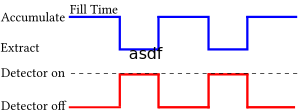
\includegraphics[width = 0.9\textwidth]{main/StoragePulse.pdf}
    \caption{Illustration (not to scale) of the measurement sequence used to obtain the results of this subsection. The octopole is allowed to fill with ions for variable times. The octopole is allowed to open for 2 ms, which is sufficient to let all the ions leave (see \cref{fig:bunchShape}). During the time when the octopole is open,
    the channeltron detector is turned on, to count the number of ions. For each fill time this procedure is repeated 20 times}
    \label{fig:storageSequence}
\end{figure}
All measurements for this experiment were taken at an ion current of approx 300 ions/second, measured at the channeltron detector.
The ion current measured at the detector usually varies within 10\% due to fluctuations in flow from the electrospray. Thus, any measurements of how long it takes to fill the octopole have to be adjusted for the ion flux during the loading phase.  This adjustment is done by multiplying the physical loading time by the ratio between the reference of 300 ions/s and the mean of the measured current before and after the experiment giving
\begin{equation}
    \tau'= \frac{I_{reference}}{I_{measured}}\tau,\quad I_{measured} = \frac{I_{before}+I_{after}}{2}.
\end{equation}
Results from the experiment with the time-axis adjsuted as described above can be seen on \cref{fig:fillTimeGraph}. From this we can make a very rough estimate of the ion current entering the octopole.
The density of ions in an octopole, where space-charge effects are included, can be written \textcolor{red}{CITE MAJIMA}
\begin{equation}
    n(r) = \frac{144\epsilon_0 V_{RF}^2}{m\Omega^2r_0^4}\bigg(\frac{r}{r_0}\bigg)^4,
\end{equation}
where $V_{rf}$ is the RF voltage of the octopole (170V), $m$ is the mass of the ion (479 amu), $\Omega$ is the frequency of the octopole RF voltage ($2\pi\times2.7$MHz) and $r_0$ is half the distance between opposing octopole rods (2.75mm).


In order to get the linear density one has to integrate this in the radial plane.
It is of course important to ensure that we integrate out to the right distance from the center axis. Gerlich suggests that the ions can be stored out to $r = 0.8r_0$, by geometric considerations \textcolor{red}{GERLICH}. We use this as it is an easy bound to implement. However the cutoff radius of the ion cloud might become more complex to describe when we are in the 
space-charge dominated regime \textcolor{red}{CITE MAJIMA}, as is the case when the octopole is full. We find the number of ions held in the octopole (length of 133mm) to be
\begin{equation}
    N = \frac{48\pi\epsilon_0V_{RF}^2L}{m\Omega^2r_0^2}\bigg(\frac{4}{5}\bigg)^6\approx 7.77\times 10^8.
\end{equation}
Again this number is likely to be lower in reality, but gives a ballpark figure for the number of ions that can be stored in the trap. Assuming the trap is full after 45 seconds of accumulation, we find there is a current of approx. $17\times 10^6$ ions/s entering the octopole while the electrospray is turned on.


\begin{figure}
    \centering
    \includegraphics[width = 0.8\textwidth]{main/FillingTimeGraph.pdf}
    \caption{Results of the measurement of filling time of the octopole. For very low fill times there seems to be a very rapid increase in signal, which then becomes linear until approx. 15 seconds. After this the curve starts tapering off as the number of ions in the detector starts capping out in the mid-late 40s range}
    \label{fig:fillTimeGraph}
\end{figure}
\subsection{Storage time of the octopole}
The final measurement that has been performed on the first octopole aims to determine the period of time, in which ions can be kept in the octopole. Since the the electrospray setup is open to atmosphere, the pumps in the setup have to work hard to ensure low pressure at the end of the setup.
If the ions can be stored in the octopole for sufficiently long periods of time, that experiments may be performed using only the ions stored in the octopole, then it is possible to plug the opening of the electrospray, allowing for better vaccuum in the system.

In order to measure the lifetime of ions stored in the octopole, we allow the ions to accumulate in the octopole for 25 seconds after which we turn off the ion current into the octopole, by increasing the voltage on the skimmer to 200V.
An illustration of the experimental sequence can be found on \cref{fig:decaySequence}.
\begin{figure}[h]
    \centering
    \includegraphics[width = 0.7\textwidth]{main/decayPulse.pdf}
    \caption{Illustration of the experimental sequence for measuring lieftime of ions in the octopole. The octopole (blue) is set to its accumulation voltage initially. The skimmer (green) is set to a low voltage of 40V for 25 seconds, allowing ions to enter the octopole. After 25 seconds have passed a voltage of 200V is applied to the skimmer. This blocks ions from entering the octopole.
    The ions are then kept in the octopole for a time, which is varied for each measurement, after which the ions are released and measured at the detector (red). Measurement is only performed once for the majority of timestamps.}    
    \label{fig:decaySequence}
\end{figure}
\begin{figure}[h]
    \centering
    \includegraphics[width = 0.8\textwidth]{main/DecayTimes.pdf}
    \caption{Measurements of the lifetime of ions in the octopole. There clearly appear to be two timescales. At the short timescale (see inset), the number of ions in the octopole appear to be decaying with a half-life on the order of magnitude of minutes (dashed-dotted line). Conversely for longer timescales the rapid decay is no longer present and instead the population in the trap is decaying on the scale of hours (dahsed line).
    The cause for the initial rapid loss of population is likely ion-ion collisions within the trap, as the internal dynamics in the trap are initially dominated by space-charge effects. Eventually the ion density becomes sufficiently low to the point where the ions no longer feel one another, and instead losses are dominated by collisions with the background gas.}
    \label{fig:decayResults}
\end{figure}
Experimental results are seen on \cref{fig:decayResults}. From the figure it is evident, that there are two timescales at play, when determining the lifetimes of the ions.
For the first two minutes there is a rapid loss of ions, which if fitted to an exponential curve leads to a half of $359\pm249$s. After the heavy losses in the first few minutes the curve flattens out considerably. If an exponential decay is fitted to this part of the data a half life of $5243\pm2782$s is obtained. The reason for the large uncertainties in the half lives is that the statistics for the data aren't very good. Especially for the measurements at high storage times, data acquisition times become prohibitve
as a single measurement takes an upwards of an hour.

The fact that there are two timescales at play indicates that space-charge effects are important when the octopole is full. A possible explanation for why the ions die off as they do, is that initially the ions are experiencing ion-ion collisions, causing heavy losses on the time-scale of minutes.
As more and more ions are lost, the density within the octopole drops to a point, where ion-ion interactions no longer dominate losses in the octopole.
At this point the losses will be largely due to ion collisions with the neutral background gas. The measurements indicate that the timescale of this process is on the scale of hours.
Thus, it will likely be possible to use the octopole as an ion storage device, allowing for the closing of the electrosapray after an initial loading.
Closing off the electrospray to atmosphere is even likely to improve the storage time in the octopole since the long-term storage is determined by collisions with atmospheric air. The lower pressure obtained when the electrospray should lower the rate of collisions, and thus further minimize losses.